\documentclass[12pt,a4paper]{article}
\usepackage[utf8]{inputenc}
\usepackage[spanish]{babel}
\usepackage{amsmath}
\usepackage{amsfonts}
\usepackage{amssymb}%simbolos matematicos
\usepackage{graphicx}
\usepackage{kpfonts}
\usepackage{hyperref}%Permite poner links
\usepackage[left=2cm,right=2cm,top=2cm,bottom=2cm]{geometry}
\usepackage{fancyhdr}
\graphicspath{{pictures/}}%Reconoce el lugar donde almaceno las fotos
\author{Leonela Alvarez Coello$^1$}
\begin{document}
\title{Ingeniería en la industria alimentaria}
\maketitle
1.  Estudiante de Darwin Eventur 


\begin{abstract}
Repositorio:\\
\url{https://github.com/091702/Proyecto_final.git}\\

El proyecto que se plantea en este Trabajo de Fin de estudiar la ingeniería en alimentos con diferentes algoritmos útiles para la optimización de procesos en la industria alimentarias, que cada día crece siendo una rubro económico importante para las naciones, se presentan  modelos planteados que son una herramienta muy necesaria para el diseño de equipos industriales. Demostrando  generalmente lo industrial real en el ámbito del tratamiento de alimentos mediante técnica. Se quiere estudiar la forma geométrica para la eficiencia y evaluar aspectos importantes para contrarrestar fallas.\\

\textbf{Palabras claves :} Ingeniería, alimentos, resoluciones, optimización. 
\end{abstract}


\newpage

\renewcommand{\contentsname}{Índice}
\tableofcontents
\newpage
\pagestyle{fancy}
\fancyhead{} 
\fancyhead[C]{Ingeniería \textit{en Alimentos}} 
\renewcommand{\headrulewidth}{0.25pt} 

\begin{center}
\section{Introducción}
\end{center}
Un alimento es cualquier sustancia o producto que, por sus características, aplicaciones y/o preparación, sirve para la nutrición humana normal, pueden ser tanto de origen animal (carne, pescado, leche, huevos) como de origen vegetal (cereales, frutas, verduras) \cite{Luzt1979}. \\

Los alimentos nos aportan nutrientes y energía (expresada en kilocalorías). Hablamos de kilocalorías (kcal) como medida de la cantidad de energía que aportan los alimentos. Cuando hay un exceso o defecto en el aporte de energía, se producen enfermedades en el organismo \cite{Rosenauer2002}. \\

Para comprender mejor la diferencia entre lo que es un nutriente y lo que es un alimento, se puede decir que los alimentos son los “envases” de los nutrientes. Los alimentos tienen diferentes tipos de nutrientes; por eso es tan importante que la alimentación sea variada\cite{Montes2005}.\\ 

Algunos nutrientes se encuentran en grandes cantidades en la comida, por eso se les denomina macronutrientes; es el caso de las proteínas, los hidratos de carbono y las grasas o lípidos. En los alimentos también hay presentes otras sustancias en muy pequeña cantidad: son los micronutrientes, como las vitaminas y los minerales \cite{Luzt1979}.\\

Actualmente la industria de alimentos está cobrando fuerza debido al crecimiento de población, creciendo demandas para alimentar constantemente, ayudando a conservar de manera inocua, calidad sensorial y nutricional, creando metodologías y formas para lograr el objetivo. ver figura \ref{fig:ali} \\

\begin{figure}[h!]
\centering
\includegraphics[width=7cm]{ali}
\caption{Ingeniería en Alimentos}
\label{fig:ali}
\end{figure}
\newpage
\section{Materiales y métodos}
\subsection{Optimización matemática en procesos industriales}
La eficiencia de cualquier tratamiento depende de la adecuada elección de ciertas variables del proceso, algunas de estas variables pueden ser la temperatura, el tiempo, la fuerza del campo eléctrico o la energía de entrada\cite{Sacancela2000}. \\

También las variables propias de los materiales a procesar, como la conductividad eléctrica del producto alimnetario a procesar.\cite{Ibarz2005} La fuerza de los campos eléctrico es comúnmente estudiada como la variable principal del proceso industrial y puede ser estimada mediante la siguiente ecuación:\\

\begin{equation}
E= \frac{V}{h}
\end{equation}

Donde V (kV) es el voltaje aplicado y h (cm) es la distancia entre los electrodos. 
\begin{equation}
Q_{spec} = m^{-1} * f* \int_{0}^{\infty} * \sigma (T)* (E(T))^2 dt,
\end{equation}
Donde:  \begin{equation}
\sigma (T) \frac{J}{s*k*m}
\end{equation} 
es la conductividad media dependiente de la temperatura.
 T (K), f es la frecuencia del pulso y m es el índice de flujo másico (kg/s). La fuerza eléctrica requerida para la pasterización de un líquido ver figura\ref{fig:ing}.\\
 
\begin{figure}[h!]
\centering
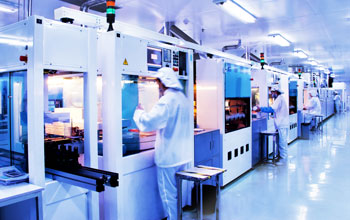
\includegraphics[width=5cm]{ing}
\caption{Procesos en la industria}
\label{fig:ing}
\end{figure}
\newpage
\subsection{Aplicaciones  de la ingeniería}
La ingeniería y la matemática están estrechamente vinculadas debido a que los conocimientos matemáticos son algunas de las herramientas fundamentales con que los ingenieros analizan, evalúan y resuelven muchos de sus problemas o proyectos, como el siguiente ejemplo: \\

\begin{equation}
V = \int_{0}^{2\phi} \int_{0}^{\phi} \int_{0}^{r} r^2 sen r^2sen(\theta)\ dr d \theta d\varphi
\end{equation}
Fuente:\cite{Sacancela2000}\\

Para los estudiantes de ingeniería industrial la derivada constituye uno de los conceptos fundamentales a aprender y a aplicar, por sus aplicaciones para la evaluación del comportamiento de modelos matemáticos representativos de situaciones reales, como es el caso de análisis de rapidez de variación, tasa de cambio, sensibilidad, optimización, análisis de curvas, etc. ver figura \ref{fig:casco} \\

\begin{figure}[h!]
\centering
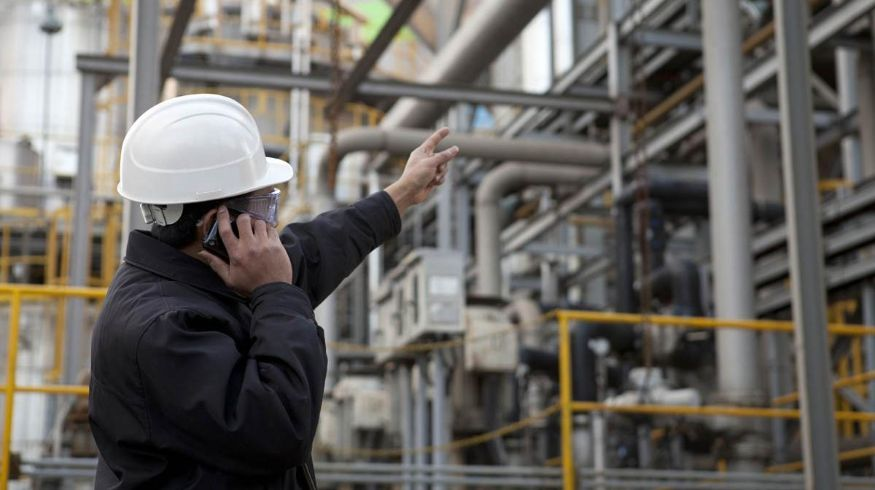
\includegraphics[width=5cm]{casco}
\caption{Aplicaciones en la industria}
\label{fig:casco}
\end{figure}
\section{Discución}
\subsection{Aplicaciones a flujo de calor en estado estacionario}
La curva punteada del tubo es una curva isotérmica. Los planos correspondientes de la pared y los cilindros se llaman superficies isotérmicas \cite{Yunus2007}. ver figura \ref{fig:images}\\

Ejemplo aclaratorio: Se calienta agua a la temperatura del punto de ebullición de Te. El agua se agita y se guarda en un cuarto el cual está a una temperatura constante de Tc. Después de ti la temperatura del agua es Tf \cite{Alvarez2005}. \\

 En el caso general, las curvas isotérmicas no serán líneas o círculos, como en los ejemplos, pero pueden ser una familia de curvas como se muestra en la siguiente figura (curvas punteadas) \cite{Campell2004} ver Tabla 1.\\
 \newpage
 
\begin{figure}[h!]
\centering
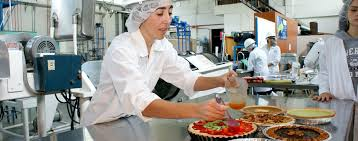
\includegraphics[width=7cm]{images}
\caption{Aplicaciones del flujo}
\label{fig:images}
\end{figure}


\begin{center}
Tabla 1. Dimensiones importantes del calor
\end{center}
\begin{minipage}[b]{1.0\linewidth}
\framebox[0.5\linewidth][c]{Unidades necesarias} \hfill \framebox[0.5\linewidth][c]{Medidas}
\framebox[0.5\linewidth][c]{Temperatura} \hfill \framebox[0.5\linewidth][c]{T °C}
\framebox[0.5\linewidth][c]{Volumen específico}  \hfill  \framebox[0.5\linewidth][c]{$m^3/kg$}
\framebox[0.5\linewidth][c]{Conductividad térmica}  \hfill  \framebox[0.5\linewidth][c]{$\frac{w}{m}$}
\framebox[0.5\linewidth][c]{Resistencia térmica }  \hfill  \framebox[0.5\linewidth] [c]{K/W}
\framebox[0.5\linewidth][c]{Viscosidad cinemática } \hfill \framebox[0.5\linewidth][c]{$m^2/s$}
\framebox[0.5\linewidth][c]{Volumen} \hfill \framebox[0.5\linewidth][c]{$m^3$}
\framebox[0.5\linewidth][c]{Velocidad} \hfill \framebox[0.5\linewidth][c]{m/s}
\framebox[0.5\linewidth][c]{Calor de vaporización del agua } \hfill \framebox[0.5\linewidth][c]{$h_{fg}$}
\framebox[0.5\linewidth][c]{Constante de Stefan-Boltzmann} \hfill \framebox[0.5\linewidth][c]{$\sigma$}\\

Fuente:\cite{Yunus2007}\\
\end{minipage}

\section{Aplicaciones a problemas combinados de crecimiento y decrecimiento}
La ecuación diferencial:
\begin{equation}
\underbrace{ay = \dfrac{dx}{dy}} 
\end{equation}
Nos dice que la variación con el tiempo de una cantidad y es proporcional a y. Si la constante de proporcionalidad a es positiva \cite{Levenspiel2004}. Ver figura \ref{fig:proceso} \\

\begin{figure}[h!]
\centering
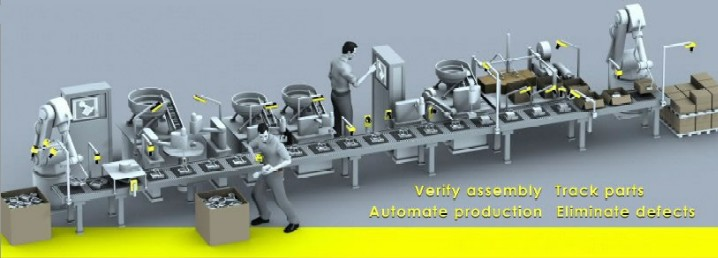
\includegraphics[width=7cm]{proceso}
\caption{Area de proceso de alimentos}
\label{fig:proceso}
\end{figure}
\newpage
\bibliographystyle{apalike}
\bibliography{bibliografi}
\end{document}